\chapter{Постоянный ток}

\section{Понятие тока}

    \begin{definition}
        \textbf{Электрический ток} -- упорядоченное движение электрических
        зарядов, то есть это явление зарядопереноса.
    \end{definition}
    
    \begin{figure}[b!]
        \center
        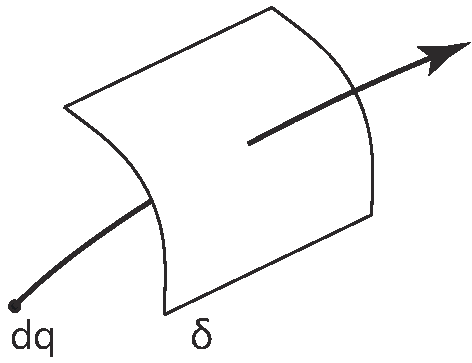
\includegraphics[width=0.47\textwidth]{lec06/current.pdf}
        \hfill
        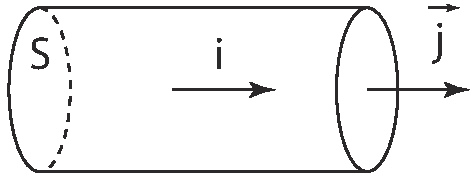
\includegraphics[width=0.47\textwidth]{lec06/steady_density.pdf}
        \parbox[t]{.47\textwidth}{\caption{Электрический ток}}
        \hfill
        \parbox[t]{.47\textwidth}{\caption{Плотность электрического тока}}
    \end{figure}
 
    \begin{figure}[t!]
        \center
        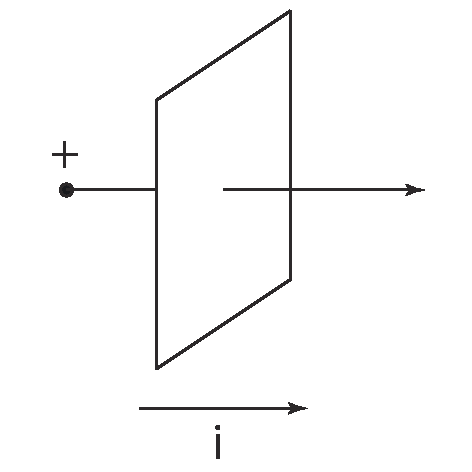
\includegraphics[width=0.47\textwidth]{lec06/cur_dir_+.pdf}
        \hfill
        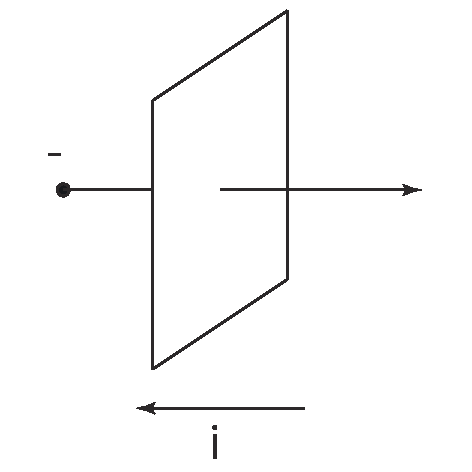
\includegraphics[width=0.47\textwidth]{lec06/cur_dir_-.pdf}
        \parbox[t]{.47\textwidth}{\caption{За направление протекания тока
            принимается направление движения положительных зарядов}}
        \hfill
        \parbox[t]{.47\textwidth}{\caption{Если носителями тока являются
                            отрицательно заряженные частицы, то ток течёт
                            в сторону, противоположную движению носителей}}
    \end{figure}

    Если через площадку \( S \) переносится заряд \( dq \) за время \( dt \),
    то ток через эту площадку:
    \[
        i = \frac{dq}{dt} \left(\frac{\text{Кл}}{\text{с}}\right),
    \]
    \[
        [i] = 1\text{ А}.
    \]
    
    То есть \( i = 1 \) А -- это ток, который переносит заряд \( q = 1 \) Кл
    за время \( \Delta t = 1 \) с. Ампер является основной единицей в СИ, и
    единица измерения электрического заряда может быть представлена в виде
    \[
        1 \text{ Кл} = 1 \text{ А} \cdot 1 \text{ с}.
    \]

    Ток -- это скалярная алгебраическая величина. Условно за направление тока
    принимается направление движения положительных зарядов \( +q \).
    
    
   
\section{Плотность тока}

    Если ток \( i \) распределен по сечению проводника равномерно, то
    \textit{плотность тока} равна отношению тока, протекающего по проводнику
    к площади поперечного сечения проводника:
    \[
        j = \frac{i}{S} \left( \frac{\text{А}}{\text{м}^2} \right).
    \]
    
    Однако, при произвольном распределении \( i \) по сечению определение
    плотности тока \( j \) должно быть несколько иным, более общим.
    Установим его.
    
    Пусть \( e \) -- заряд носителя, \( \vec{v_i} \) -- тепловые скорости
    хаотического движения свободных носителей, а  \( \vec{E} \) -- поле,
    приложенное к проводнику. В случае \( \vec{E} = 0 \)
    \[
        \sum\limits_i \vec{v_i} = 0,
    \]
    зарядопереноса нет, следовательно, ток через любую поверхность \( S \)
    равен нулю.
    \begin{align*}
        & \frac{m v_i^2}{2} = \frac{3}{2}kT, \\
        & k = 1.38 \times 10^{23} \frac{\text{Дж}}{\text{с}}, \\
        & T = 300 \text{К}, \\
        & v_i = \sqrt{\frac{3kT}{m_e}} \approx 100 \frac{\text{км}}{\text{с}}.
    \end{align*}
    
    Если к проводнику приложить \( \vec{E} \ne 0 \), то движение свободных
    зарядов станет \textit{слегка} упорядоченным.
    \begin{figure}[t!]
        \center
        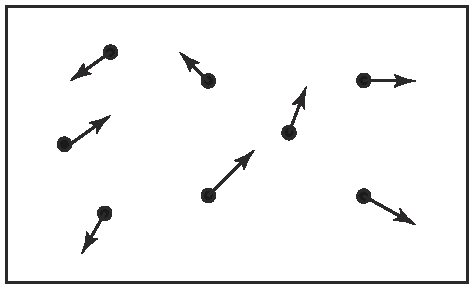
\includegraphics[width=.47\textwidth]{lec06/thermal_motion.pdf}
        \hfill
        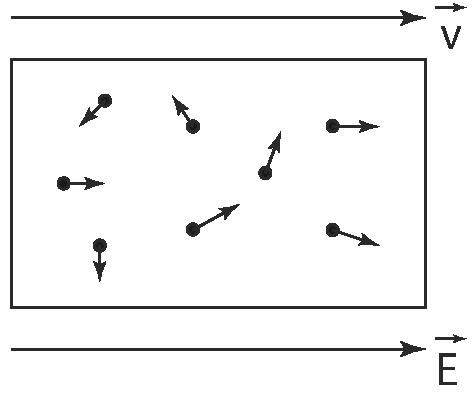
\includegraphics[width=.47\textwidth]{lec06/drift.pdf}
        \parbox[t]{.47\textwidth}{\caption{Электроны в проводнике в отсутствие
        внешнего электрического поля}}
        \hfill
        \parbox[t]{.47\textwidth}{\caption{Если внутри проводника создать поле,
        то электроны начнут дрейфовать}}
    \end{figure}
    \begin{figure}[b!]
        \center
        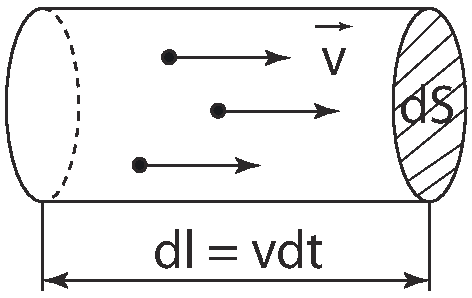
\includegraphics[width=.47\textwidth]{lec06/density_calc.pdf}
        \hfill
        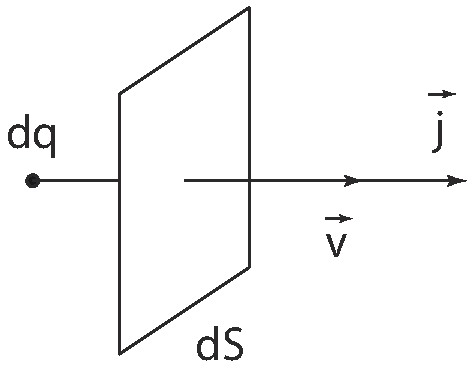
\includegraphics[width=.47\textwidth]{lec06/density_def.pdf}
        \parbox[t]{.47\textwidth}{\caption{К рассчёту плотности электрического
        тока}}
        \hfill
        \parbox[t]{.47\textwidth}{\caption{К определению плотности
        электрического тока}}
    \end{figure}
    \begin{definition}
        Средняя скорость упорядоченного движения свободных зарядов называется 
        \textbf{дрейфовой}.
    \end{definition}
    \begin{equation}
        \vec{v_{\textit{др}}} = \frac{1}{N}\sum\limits_k \vec{v_k},
    \end{equation}
    где \( \vec{v_k} \) -- скорость отдельного заряда. В дальнейшем будем
    обозначать дрейфовую скорость за \( \vec{v} \).
    
    Пусть в проводнике \( \vec{v} \ne 0 \). Построим на векторе \( \vec{v} \)
    прямой цилиндр. По определению, за время \( \dd t \) все заряды внутри этого
    цилиндра \( \dd V = \dd S\dd l = \dd S v \dd t \) пересекут его передний
    торец. Их количество в цилиндре \( \dd N = n\dd V = nv\dd S\dd t \),
    где \( n \) -- концентрация свободных носителей в проводнике.
    
    \begin{definition}
        Векторная величина \( \vec{j} \), показывающая направление
        зарядопереноса и равная заряду, переносимому за время \( dt \) через
        площадку \( \dd S \), перпендикулярную направлению зарядопереноса,
        называется \textbf{плотностью тока}.
    \end{definition}
    
    \[
        \vec{j} = \frac{\dd q}{\dd t\dd S}\vec{n}.
    \]

    А так как \( \dd q = e\dd N \), где \( e \) -- заряд носителя, а
    \( \dd N = n \dd V = nv \dd S \dd t \), то
    \begin{equation}
        \vec{j} = \frac{\dd q}{\dd t\dd S}\vec{n} =
        ne\vec{v} \left( \frac{\text{А}}{\text{м}^2} \right)
        \label{eq6:1}
    \end{equation}
    
    Тогда, ток \( i \) через поверхность \( S \) определяется как поток
    \( \vec{j} \):
    \[
        i = \iint\limits_S \vec{j}\cdot\vec{\dd S}.
    \]
    
    Если зарядоперенос осуществляется зарядами обоих знаков, то:
    \[
        \vec{j} = n_{+}e_{+}\vec{v_{+}} + n_{-}e_{-}\vec{v_{-}} =
        e_{+}[n_{+}\vec{v_{+}} - n_{-}\vec{v_{-}}]
    \]
    
    \begin{example}
        Пусть по медному проводнику сечением \( S = 1 \text{мм}^2 \) идет ток
        \( i = 1 \text{А} \). Вычислить дрейфовую скорость электронов.
    \end{example}
    
    \begin{solution}
        \begin{align*}
            & j = nev = \frac{i}{S}, \\
            & v = \frac{i}{neS}.
        \end{align*}
        Подставляя значения получим:
        
        \[
            v = \frac{1 \text{А}}{10^{29} \frac{\text{шт}}{\text{м}^3} \cdot
            1,6 \cdot 10^{-19} \text{Кл} \cdot 10^{-6} \text{м}^2} \approx
            10^{-4} \frac{\text{м}}{\text{с}} = 0,1 \frac{\text{мм}}{\text{с}}
        \]
        \begin{comment}
            Концентрация свободных зарядов \( n \) может быть получена из
            следующих соображений:
            \begin{align*}
                & n = \frac{N}{V}, \\
                & \frac{m}{M} = \frac{N}{N_A}, \\
                & N = N_A\frac{m}{M}, \\
                & n = \frac{N_A}{M}\frac{m}{V} = \frac{N_A}{M}\rho,
            \end{align*}
            где \( \rho \) -- плотность вещества, \( N_A \) -- число Авогадро,
            \( M \) -- молярная масса.
        
            Для меди
            \[
                n \approx 10^{29} \left(\frac{\text{шт}}{\text{м}^3}\right).
            \]
        \end{comment}
    \end{solution}
    
\section{Закон сохранения заряда}

    В изолированной системе \( \sum \pm q_i = \const \). Рассмотрим замкнутую
    поверхность \( S \), в которой есть некоторый заряд, и он истекает из
    \( S \).
    \begin{figure}[b!]
        \center
        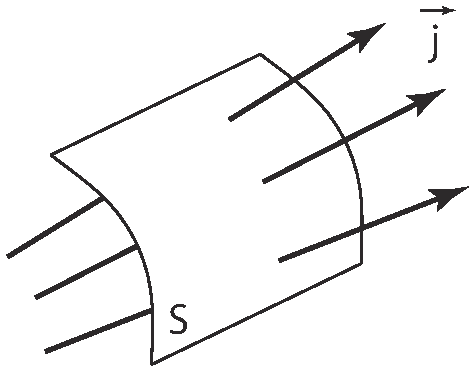
\includegraphics[width=0.47\textwidth]{lec06/flux_j.pdf}
        \hfill
        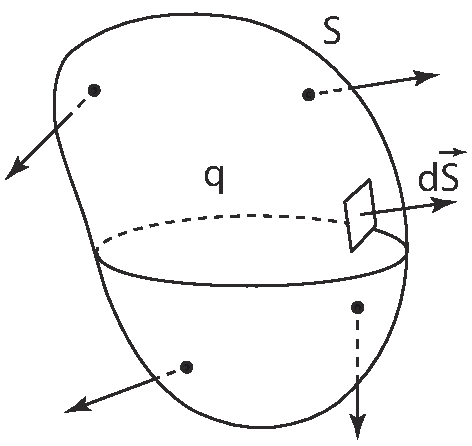
\includegraphics[width=0.47\textwidth]{lec06/emission.pdf}
        \parbox[t]{.47\textwidth}{\caption{Ток -- это поток плотности тока
                                                        через поверхность}}
        \hfill
        \parbox[t]{.47\textwidth}{\caption{Закон сохранения заряда}}
    \end{figure}
    
    Скорость убывания заряда в \( S \):
    \begin{equation}
        -\frac{\dd q}{\dd t} = i_S = \oiint\limits_S \vec{j}\cdot\vec{\dd S}
        \label{eq6:2}
    \end{equation}
    
    Итак, формула (\ref{eq6:2}) и выражает закон сохранения заряда в
    интегральном виде: заряд внутри области \( V \) может изменятся только
    путем втекания или истекания заряда через её границу \( S \).
    
    Если заряд \( q \) распределен в области \( V \) непрерывно, то
    \[
        q = \iiint\limits_V \rho \dd V.
    \]
    По теореме Остроградского:
    \[
        \oiint\limits_S \vec{j}\cdot\vec{\dd S} =
        \iiint\limits_V \div\vec{j}\dd V.
    \]
    В силу произвольности \( V \) и \( S \) подынтегральные выражения равны:
    \begin{equation}
        -\frac{\partial\rho}{\partial t} = \div\vec{j}
        \label{eq6:2a}
    \end{equation}
    
    Уравнение (\ref{eq6:2a}) описывает закон сохранения заряда в
    дифференциальной форме. Если \( \rho(x, y, z) = \const_t \), то
    \( \div\vec{j} = 0 \), и, следовательно, поле \( \vec{j} \) --
    соленоидальное, то есть линии его замкнуты. Если же
    \( \rho = \rho(x, y, z, t) \), то  \( \div\vec{j} \ne 0 \), и
    \[
        \oiint\limits_S \vec{j}\cdot\vec{dS} = -\frac{dq}{dt} \ne 0
    \]
    
\section{Закон Ома}

    Экспериментально обнаружено, что для некоторых проводников, при не слишком
    больших полях, не слишком высоких частотах, не слишком низких температурах,
    ток \( i \) пропорционален разности потенциалов \( \Delta \varphi \):
    \[
        U = Ri,
    \]
    где \( R \) -- коэффициент пропорциональности между током и напряжением,
    являющийся характеристикой \textit{образца}, называемый
    \textbf{сопротивлением} проводника:
    \begin{equation}
        R = \frac{U}{i} \left( \text{Ом} \right).
    \end{equation}
    
    Для цилиндрического проводника его сопротивление \( R \) прямо
    пропорционально его длине \( l \) и обратно пропорционально его площади
    поперечного сечения \( {S} \):
    \[
        R = \rho\frac{l}{S},
    \]
    где \( \rho \) -- \textbf{удельное сопротивление} проводника, являющееся
    характеристикой \textit{материала}.
    
    Величина 
    \[
        \lambda = \frac{1}{\rho} [\text{Ом}\cdot\text{м}]^{-1}
    \] 
    называется \textbf{удельной проводимостью} материала. Для лучших
    проводников (\( Ag, Au, Cu, Al \))
    \( \lambda \sim 10^8 (\text{Ом}\cdot\text{м})^{-1} \).
    
\section{Соединение резисторов}
    \begin{figure}[b!]
    \center
    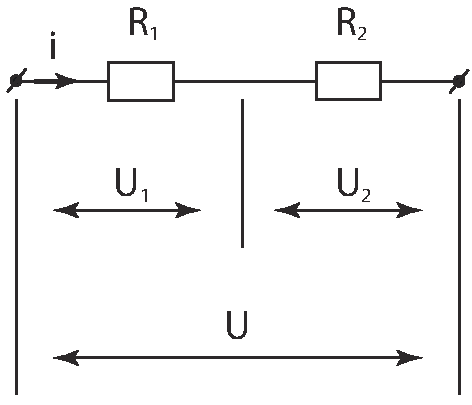
\includegraphics[width=0.47\textwidth]{lec06/R_serial.pdf}
    \hfill
    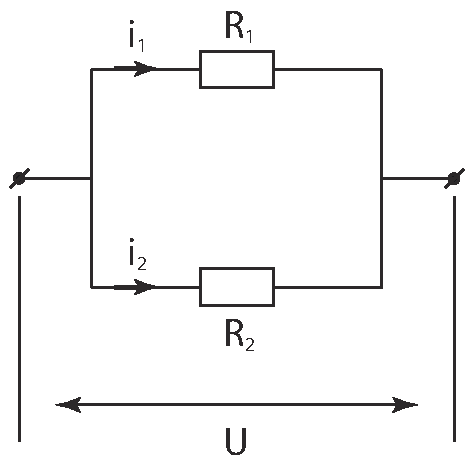
\includegraphics[width=0.47\textwidth]{lec06/R_parallel.pdf}
    \parbox[t]{.47\textwidth}{\caption{Последовательное соединение
                                                        резисторов}}
    \hfill
    \parbox[t]{.47\textwidth}{\caption{Параллельное соеднение резисторов}}
    \end{figure}

    Физическим элементом, выполняющим роль сопротивления, является
    \textit{резистор}.Рассмотрим некоторые способы соединения резисторов:
    
    \begin{enumerate}
        \item Последовательное соединение:
        \begin{align*} 
        & \left\{
        \begin{array}{rl}
            U_{ab} = & U_1 + U_2, \\
            i_{ab} = & i_1 = i_2,
        \end{array} \right. \\
        & R_{ab} = R_1 + R_2.
        \end{align*}
        \item Параллельное соединение:
        \begin{align*} 
        & \left\{
        \begin{array}{rl}
            U_{ab} = & U_1 = U_2, \\
            i_{ab} = & i_1 + i_2,
        \end{array} \right. \\
        & \frac{1}{R_{ab}} = \frac{1}{R_1} + \frac{1}{R_2}. \nonumber
        \end{align*}
    \end{enumerate}
    
\section{Закон Ома в дифференциальной форме}

    Применим закон Ома к бесконечно малому цилиндрическому элементу проводника.
    Пусть к бесконечно малому проводнику длины \( \dd l \) с поперечным
    сечением \( \dd S \) сопротивлением \( \dd R \) приложено напряжение
    \( \dd U \), и в нём протекает ток \( \dd i \):
    \[
        \left\{
        \begin{array}{l}
            \dd i = j\dd S, \\
            \dd U = E\dd l, \\
            \dd R = \rho\frac{\dd l}{\dd S}.
        \end{array}
        \right.
    \]
    
    Подставим это в закон Ома
    \[
        \dd i = \frac{\dd U}{\dd R}
    \]
    и получим:
    \[
        j = \frac{1}{\rho} E.
    \]
    Или, в векторном виде (\( \vec{j} \uparrow\uparrow \vec{E} \)):
    \begin{equation}
        \vec{j} = \lambda \vec{E}.
    \end{equation}
    Это и есть закон Ома в дифференциальном виде.
    
\section{Закон Джоуля-Ленца}

    Рассмотрим проводник. Так как ток \( i \) -- это явление зарядопереноса,
    то для переноса очередной порции заряда \( \dd q \) с левого конца
    проводника на правый поле \( \vec{E} \) по определению должно совершить
    работу
    \[
        \dd A = U\dd q = (\varphi_1 - \varphi_2)\dd q.
    \]
    
    А так как \( \dd q = i\dd t \), то \( \dd A = iU\dd t \). Эта работа
    превращается в тепло \( \dd Q \), выделяющееся в проводнике, так как к концу
    пути заряды не приобретают дополнительной скорости:
    \begin{equation}
        \dd Q = iU\dd t.
        \label{eq:dQ}
    \end{equation}
    
    \begin{definition}
        Величину
        \[
            P = \frac{\dd Q}{\dd t} \left(\frac{\text{Дж}}{\text{с}} =
            \text{Вт}\right)
        \]
        называют \textbf{тепловой мощностью}, выделяемой в проводнике.
    \end{definition}
    
    Полученное выше выражение (\ref{eq:dQ}) может быть записано в виде
    \begin{equation}
        P = iU.
    \end{equation}
    Полученное выражение есть ни что иное, как математическая запись закона
    Джоуля-Ленца. Так как \( U = iR \), то:
    \[
        P = i^2 R = \frac{U^2}{R}.
    \]
    
    Применим закон Джоуля-Ленца к бесконечно малому элементу проводника.
    \[
        \dd P = \dd i\dd U = j\dd SE\dd l = jE\dd V,
    \]
    где \( \dd V \) -- объем бесконечно малого проводника.
    
    \begin{definition}
        Величина
        \[
            p = \frac{dP}{dV} \left(\frac{\text{Вт}}{\text{м}^3}\right)
        \]
        называется \textbf{плотностью тепловой мощности}.
    \end{definition}
    
    Таким образом,
    \begin{equation}
        p = jE.
    \end{equation}
    А так как \( j = \lambda E \), то
    \[
        p = \lambda E^2 = \frac{1}{\lambda}j^2 = \rho j^2.
    \]
    Это закон Джоуля-Ленца в дифференциальном виде. Тогда тепло, выделившееся
    в проводнике:
    \[
        Q = \int\limits_0^t \left(
            \iiint\limits_V p(x, y, z, t)\dd V
            \right) \dd t.
    \]
    
\section{Электродвижущая сила (ЭДС)}
    
    Для того, чтобы поддерживать в проводнике ток, необходимо каким-либо образом
    переносить заряды \( +q \) с правого конца с низким потенциалом
    \( \varphi_1 \) к концу с высоким потенциалом \( \varphi_2 \), то есть
    осуществлять постоянный зарядоперенос. Электростатическая сила
    \( \vec{F}_{\textit{эл}} = e\vec{E} \) этого сделать не может, так как
    справеддлива теорема о циркуляции поля \( \vec{E} \)
    \[
        \oint\limits_C \vec{E}\cdot\vec{dl} = 0.
    \]
    
    Для осуществления такого зарядопереноса должна действовать какая-то другая
    сила, неэлектростатического происхождения.
    
    \begin{definition}
        Любая сила неэлектростатического происхождения (механическая,
        химическая, магнитная и др.) называется \textbf{сторонней силой}.
    \end{definition}
    \begin{definition}    
        Устройство, которое реализует зарядоперенос при помощи сторонней силы,
        называется \textbf{генератором}.
    \end{definition}
    \begin{definition}
        Работа сторонней силы по переносу заряда из точки 1 с низким
        потенциалом в точку 2 с высоким потенциалом, отнесенная к величине
        этого заряда, называется \textbf{электродвижущей силой} (ЭДС),
        действующей на участке \( 1 \rightarrow 2 \).
    \end{definition}
    
    \begin{figure}[b!]
        \center
        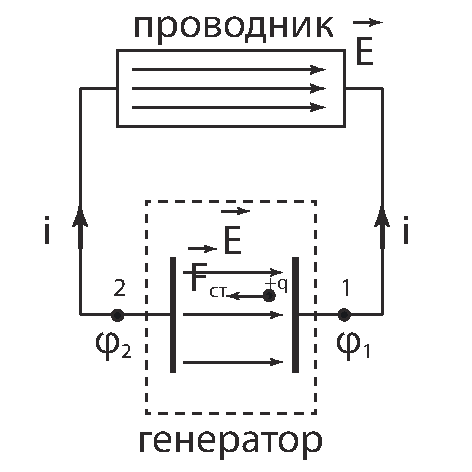
\includegraphics[width=.47\textwidth]{lec06/emf.pdf}
        \hfill
        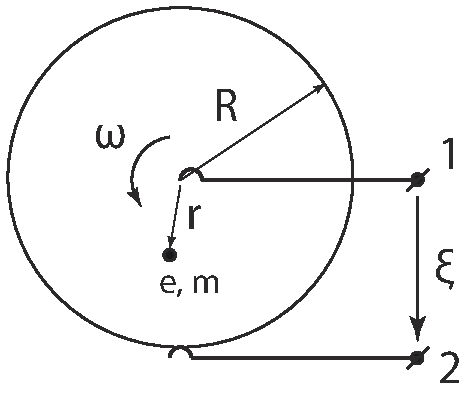
\includegraphics[width=.47\textwidth]{lec06/cuprum_disc.pdf}
        \parbox[t]{.47\textwidth}{\caption{ЭДС}}
        \hfill
        \parbox[t]{.47\textwidth}{\caption{Униполярный генератор}}
    \end{figure}
    
    Таким образом, ЭДС:
    \begin{equation}
    \EDS_{12} (\text{В}) \equiv \frac{1}{q} \int\limits_1^2
    \vec{F}_{\textit{ст}}\cdot\vec{dl}
    \end{equation}

    Сторонней силе \( \vec{F}_{\textit{ст}} \) можно сопоставить поле сторонних
    сил:
    \[
        \vec{E}_{\textit{ст}} = \frac{\vec{F}_{\textit{ст}}}{q}.
    \]
    Тогда ЭДС
    \begin{equation}
        \EDS_{12} = \int_1^2 \vec{E}_{\textit{ст}}\cdot\vec{dl}
    \end{equation}
    
    \begin{example}[Униполярный генератор]
        Медный диск радиуса \( R \) вращается со скоростью \( \omega \).
        Найти ЭДС на участке \( 1 \rightarrow 2 \).
    \end{example}
    
    \begin{solution}
    Здесь в качестве сторонней силы выступает центробежная сила\footnote{Вообще
    говоря, центробежная сила -- это сила инерции, и реально она не существует.
    Поэтому я не уверен насчёт высказывания о сторонней силе в униполярном
    генераторе. -- Абдрахманов В}:
        \[
            \vec{F}_{\textit{ст}} = \vec{F}_{\textit{цб}} = m\omega^2r.
        \]
    
        Тогда на участке \( 1 \rightarrow 2 \) действует ЭДС:
        \[
            \EDS = \frac{1}{e} \int \vec{F}_{\textit{ст}}\cdot\vec{dl} = 
            \frac{m\omega^2}{e}\int rdr = \frac{m\omega^2R^2}{2e}. \nonumber 
        \]
    
        Пусть \( R = 0,1 \text{м} \),
        \( \omega = 1000 \frac{\text{рад}}{\text{с}} \).
        Тогда
        \[
            \EDS = \frac{1}{2} \cdot 10^{-11} \cdot 10^6 \cdot 10^{-2} =
            5 \cdot 10^{-8} = 0,05 \text{мкВ}.
        \]
    \end{solution}
    \clearpage % иначе сноска уходит на другую страницу

\section{Обобщенный закон Ома}
    \begin{figure}[b!]
        \center
        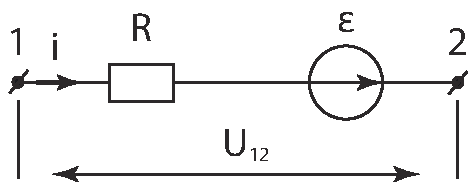
\includegraphics[width=0.3\textwidth]{lec06/generic_ohm.pdf}
        \hfill
        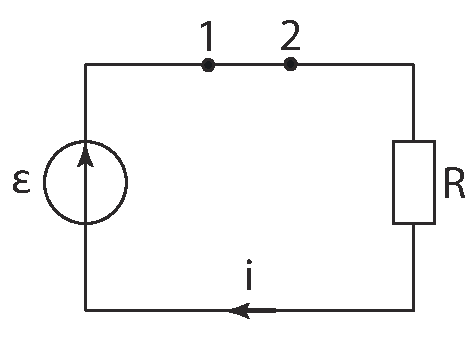
\includegraphics[width=0.3\textwidth]{lec06/closed_g_o.pdf}
        \hfill
        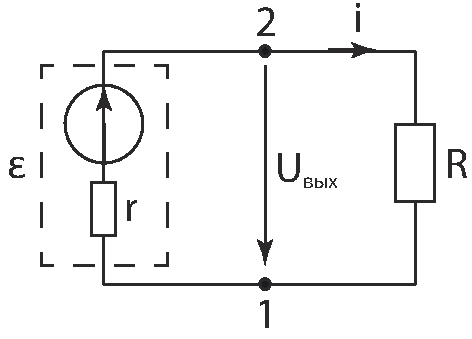
\includegraphics[width=0.3\textwidth]{lec06/U_ext.pdf}
        \parbox[t]{.3\textwidth}{\caption{Обобщённый закон Ома}}
        \hfill
        \parbox[t]{.3\textwidth}{\caption{Закон Ома для замкнутой цепи}}
        \hfill
        \parbox[t]{.3\textwidth}{\caption{Выходное напряжение}}
    \end{figure}
    Если на свободные заряды в проводнике действуют как электрические силы,
    так и сторонние, то в результате их совместного действия в проводнике будет
    протекать ток:
    \begin{equation}
        \vec{j} = \lambda (\vec{E} + \vec{E}_{\textit{ст}})
        \label{eq6:691}
    \end{equation}
    Уравнение (\ref{eq6:691}) -- обобщенный закон Ома в дифференциальном виде.
    Получим его в интегральном виде.

    Для этого рассмотрим участок цепи, содержащий резистор \( R \) и генератор
    \( \EDS \). Проинтегрируем (\ref{eq6:691}) от 1 до 2:
    \[
        \int\limits_1^2 \frac{\vec{j}\cdot\vec{dl}}{\lambda} =
        \int\limits_1^2 \vec{E}\cdot\vec{dl} + \int\limits_1^2 
        \vec{E}_{\textit{ст}}\cdot\vec{dl}.
    \]
    Так как в линейном проводнике \( \vec{j} \uparrow\uparrow \vec{E}
    \uparrow\uparrow  \vec{E}_{\textit{ст}} \uparrow\uparrow \vec{dl} \), то
    \[
        \int\limits_1^2 \rho \left( \frac{i}{S} \right)dl =
        \int\limits_1^2 Edl + \int\limits_1^2 E_{\textit{ст}} dl.
    \]
    
    Но:
    \begin{enumerate}
    \item
        По определению разности потенциалов:
        \[
            \int\limits_1^2 Edl = U_{12};
        \]
    \item
        По определению ЭДС:
        \[
            \int\limits_1^2 E_{\textit{ст}}dl = \EDS_{12};
        \]
    \item
        \[
            \int\limits_1^2 \rho \left( \frac{i}{S} \right)dl =
            i \int\limits_1^2 dR_{12} = iR 
        \]
    \end{enumerate}
    
 
    
    Таким образом, интегральная форма (\ref{eq6:691}) выглядит следующим образом:
    \begin{equation}
        iR = U_{12} + \EDS.
        \label{eq6:691a}
    \end{equation}
    
    Если цепь замкнута, то есть точка 1 совпадает с точкой 2 и \( U_{12} = 0 \),
    то получаем закон Ома для амкнутой цепи:
    \begin{equation}
        i = \frac{\EDS}{R}.
    \end{equation}
    Если сам генератор имеет внутреннее сопротивление \( r \), то закон Ома для
    замкнутой цепи будет выглядеть так:
    \begin{equation}
        i = \frac{\EDS}{R + r}.
    \end{equation}
    
    Напряжение \( U_{21} \) между выходными клеммами генератора называется его
    \textbf{выходным напряжением}: \( U_{\textit{вых}} = U_{21} \). Найдем его.
    
    Применим (\ref{eq6:691a}) к участку \( 1 \rightarrow 2 \):
    \begin{align}
        & ir = U_{12} + \EDS, \nonumber \\
        & U_{\textit{вых}} = U_{21} = -U_{12}, \nonumber \\
        & U_{\textit{вых}} = \EDS - ir.
        \label{eq6:692}
    \end{align}
    
    Лишь в режиме холостого хода (когда \( i = 0 \)) \( U_{\textit{вых}} =
    \EDS \), в других случаях \( U_{\textit{вых}} < \EDS \). Графически эта
    зависимость выглядит так:
    % тут такая прямая
    % при i = 0: U_вых = EDS
    % при U_вых = 0: i = i_короткого замыкания

    \( i_{\textit{к. з}} \approx 3 \text{А} \) у хороших батарей,
    \( \approx 100 \text{А}\) у автомобильных аккумуляторов.

\section{Правила Кирхгофа}

    Изучить по описанию \href{http://google.com}{работы Ф303}.
    
\section{Ток в безграничной слабопроводящей среде}

    Пусть в безграничной слабопроводящей среде помещены два металлических
    электрода \( A \) и \( B \) такие, что \( \lambda_{\textit{среды}} \ll
    \lambda_{\textit{мет}} \).
    Геометрия электродов задана, также дана проводимость среды
    \( \lambda_{\textit{среды}} \). Необходимо определить сопротивление среды
    по постоянному току.
    
    \begin{solution}
        
        Так как \( \lambda_{\textit{среды}} \ll \lambda_{\textit{мет}} \), то на
        поверхностях электродов \( \varphi_A = \const \) и \( \varphi_B = \const \),
        и, следовательно, линии поля \( \vec{E} \) перпендикулярны поверхности
        электродов. Так как среда предполагается однородной, то в ней
        \[
            \frac{\partial p}{\partial t} = 0.
        \]
        А так как, по закону сохранения заряда,
        \[
            \div\vec{j} = -\frac{\partial p}{\partial t},
        \]
        то в среде \( \div\vec{j} = 0 \). По закону Ома \( \vec{j} =
        \lambda\vec{E} \), тогда и \( \div\vec{E} = 0 \).

        Но в вакууме \( \div\vec{E}_0 = 0 \) и линии поля \( \vec{E}_0 \)
        перпендикулярны поверхности металла.
        
        В силу единственности решения краевой задачи, поле в среде
        \( \vec{E} \equiv \vec{E}_0 \).
        
        Далее, ток
        \[
            i = \oiint\limits_S \vec{j}\cdot\vec{dS},
        \]
        где \( S \) -- поверхность, охватывающая какой-либо электрод.
        А так как \( \vec{j} = \lambda\vec{E} \), то
        \[
            i = \lambda\oiint\limits_S \vec{E}\cdot\vec{dS} =
            \lambda\oiint\limits_S \vec{E}_0 \cdot \vec{dS}.
        \]
        Тогда, по теореме Гаусса
        \[
            i = \lambda\frac{q_S}{\varepsilon_0} = \lambda\frac{q}{\varepsilon_0},
        \]
        где \( q \) -- заряд любого из электродов.
        
        А так как, по определению емкости системы \( AB \):
        \[
            C_{AB} = \frac{q}{\Delta\varphi} = \frac{q}{U},
        \]
        то
        \[
          i = \lambda\frac{C_{AB}U}{\varepsilon_0},
        \]
        где \( C_{AB} \) -- емкость конденсатора \( AB \) в \textit{вакууме}, то
        есть \( \eps = 1 \).
        
        И тогда сопротивление среды:
        \begin{equation}
            R_{AB} = \frac{U}{i} = \frac{\varepsilon_0}{\lambda C_{AB}}.
            \label{eq6:n1}
        \end{equation}
    \end{solution}
    
    \begin{figure}[b!]
        \center
        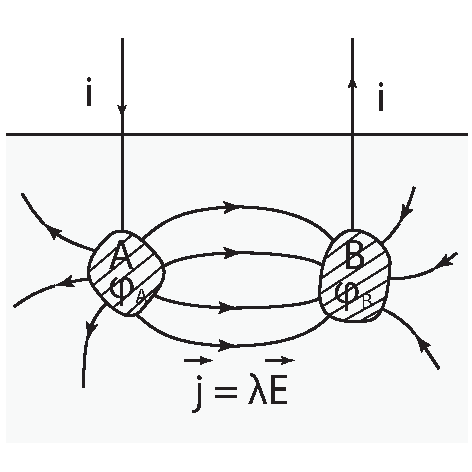
\includegraphics[width=0.3\textwidth]{lec06/inf_environment.pdf}
        \hfill
        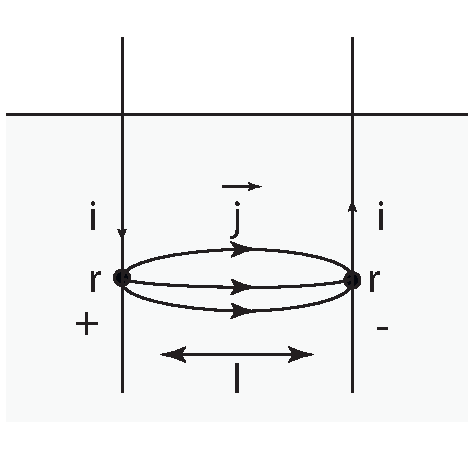
\includegraphics[width=0.3\textwidth]{lec06/2_balls.pdf}
        \hfill
        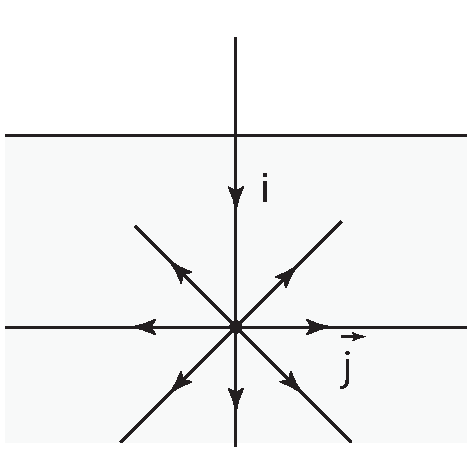
\includegraphics[width=0.3\textwidth]{lec06/ground.pdf}
        \parbox[t]{.3\textwidth}{\caption{Ток в бесконечной слабопроводящей
                                                                    среде}}
        \parbox[t]{.3\textwidth}{\caption{К примеру с шариками}}
        \parbox[t]{.3\textwidth}{\caption{Заземление}}
    \end{figure}
    
    \begin{example}
        Вычислить сопротивление \( R \) между двумя шариками радиуса \( r \),
        находящихся на расстоянии \( l \gg r \) друг от друга в земле.
    \end{example}
    
    \begin{solution}
        Вычислим емкость пары шаров:
        \[
            \varphi_1 = \frac{+q}{4\pi\varepsilon_0 r};\ 
            \varphi_2 = \frac{-q}{4\pi\varepsilon_0 r}
        \]
        Тогда
        \[
            U = \varphi_1 - \varphi_2 = \frac{q}{2\pi\varepsilon_0 r}.
        \]
        
        Так как шары далеко друг от друга и поэтому не влияют друг на друга, иначе
        бы потенциал каждого из шаров был бы равен \( \varphi_{\textit{ш}} =
        \varphi_{\textit{собст}} + \varphi_{\textit{чуж}} \). Поэтому ёмкость этой
        системы
        \[
            C = \frac{q}{U} = 2\pi\varepsilon_0 r.
        \]
        
        По формуле (\ref{eq6:n1}):
        \[
            R = \frac{\varepsilon_0}{\lambda\cdot 2\pi\varepsilon_0 r} =
            \frac{\rho}{2\pi r},
        \]
        где \( \rho \) -- удельное сопротивление среды (от \( l \) не зависит).
    \end{solution}
    
    \begin{example}
        Определить сопротивление заземления, если оно сделано в виде шара
        радиуса \( r \).
    \end{example}
    
    \begin{solution}
        Ёмкость уединённого шара
        \[
            C = 4\pi\varepsilon_0 r.
        \]
        
        Тогда по формуле (\ref{eq6:n1})
        \[
            R = \frac{1}{4\pi\lambda r} = \frac{\rho}{4\pi r}.
        \]
        Видно, что сопротивление одного шара меньше сопротивления пары.
    \end{solution}
    
    \begin{example}
        В земле проложена двухпроводная линия длины \( l \) и радиуса \( r \),
        расстояние между проводами \( d \gg r \). Определить сопротивление
        утечки в такой линии.
    \end{example}
    
    \begin{solution}
        Емкость линии
        \[
            C = \frac{\pi\varepsilon_0}{\ln\left(\frac{d}{r}\right)} l.
        \]
    
        А её сопротивление
        \[
            R = \frac{\rho}{\pi l}\ln\left(\frac{d}{r}\right).
        \]
    \end{solution}
